% !TeX root = user_guide.tex
\subsection{Databse connection}
Every time you will start \edacc you will be prompted to provide the connection data to the \mysql database you would like to work with. 
\begin{center}
	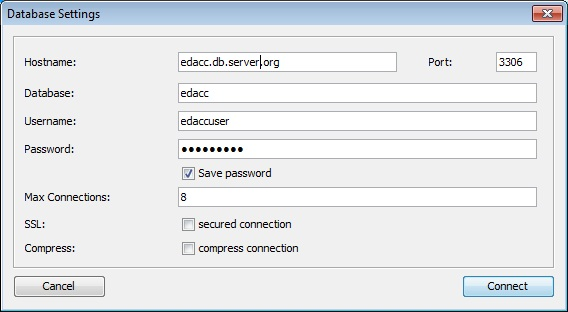
\includegraphics[width=1.00\textwidth]{snapshots/DBlogin.jpg}
\end{center}

\marginlabel{host name / IP}In the connection dialog you have to provide the host name or the IP-address of your \mysql database. 

\marginlabel{port}If you have configured the \mysql server to use an other port then the default \mysql port 3306, you can specify this in the \textbf{Port:} text field. 

\marginlabel{DB name} Further you also have to provide a valid database name and a user along with the corresponding password. 

\marginlabel{saving connection} If you would like to save the details of this connections for further usage you can check the \textbf{Save password} check-box. \edacc will save the password for you \todo in an encrypted form WO?

\marginlabel{Max Connections} \edacc is a multi-threaded program and will use more than on connection to the database to speed up certain tasks. We recommend to allow up to 8 simultaneous database connections, but if you have restrictions on this number you can specify it in the \textbf{Max Connection:} text field. 

\marginlabel{SSL connections} If you are going to use \edacc to store trusted data we strongly recommend to enable a SSL connection by checking the \textbf{secured connection} cechk box. \todo Be aware that this kind of connection is only possible is the \mysql server is configured accordingly. 

\marginlabel{Compressed Connections} When working with \edacc through a slow network connection you might want to turn on compression by checking the \textbf{compress connection} check box. 

\marginlabel{Connect} After providing all the information you can connect to the \mysql server. 

\marginlabel{Create DB} When you connect the first time to a database \edacc will create for you all the needed tables. \todo Was passiert wenn man sich an einer falschen DB verbindet, die ein anderes Modell hat. Kann man das EDACC DB Modell neu erzeugen �ber einen bestehenden? 

\marginlabel{DB Model version} 
As \edacc is under full development and the database model may be extended to support new features, \edacc will check if the database model is compatible with the GUI version. Within this check we  differentiate between two cases:
\begin{enumerate}
	\item \ml{DB Model upgrade}The database model version is to old for the GUI. In this case \edacc will offer you the possibility to upgrade your database scheme to the latest version. \todo Werden da auch mehrere versionen �bersprungen? Sprich von version 0.1 auf 0.4?
	\item \ml{GUI update}The database model version is to new for the GUI. In this case you should update the GUI. You can do this by using the automatic update function of \edacc, which can be found under \textbf{Help $\rightarrow$ Check for Updates}. Another possibility is to download the latest release form the project site at \url{http://sourceforge.net/projects/edacc/}. 
\end{enumerate}

\subsection{Manage Database Mode}

% !TeX root = managedbmode.tex
\marginlabel{Solvers} A solver is a program which implements an algorithm for solving a problem. In EDACC a solver is represented by the following information:
\begin{enumerate}
 \item[Name] A human-readable name of the solver.
 \item[Version] The version number of the solver. The combination of name and version must be unique.
 \item[Description] A short description of the solver.
 \item[Authors] The list of the authors of a solver.
 \item[Code] The sourcecode of the solver.
 \item[Several Binaries] A solver can consist of different binaries, which have the same source code but differ in the compile options (eg. the architecture) or the chosen compiler version. There must be at least one solver binary.
\end{enumerate}

\marginlabel{Parameters} Every solver has a list of several parameters which control its behaviour. To build a valid parameter list string, EDACC needs the following information:
\begin{enumerate}
 \item[name] The human-readable internal name of the parameter. This name has no effect to the generated command-line and is only needed for reasons of indentification in the EDACC system.
 \item[prefix] The parameter prefix defines how the parameter is called on the command-line. The Unix program \verb|ls| for example has a parameter with the prefix \verb|-l|.
 \item[Boolean] Some parameters don't have an actual value but act as switches for a certain functionality of a solver. The \verb|-l| parameter of the Unix program \verb|ls| for example is such a boolean parameter.
 \item[Mandatory] Some parameters need to be specified to start the solver binary. Such parameters are called mandatory.
 \item[Space]
 \item[Order] Some solvers need a special order of the parameters. This order is specified by an ascending number. The parameter with the smallest number will be used first in the command-line string. If two parameters have the same order number, the order between those two parameters doesn't matter.
\end{enumerate}

\marginlabel{Add Solver}
By clicking the button ``New'' in the solver panel a new empty line in the solver table is created. To fill the new entry with information fill in the form below the table with the static information of the solver. Optionally you can attach the code of the solver to the entry by clicking on ``Add Code'' and choosing the files or directories from your file system. 

\attention To create a valid solver entry, it is necessary to specify at least one solver binary.

\marginlabel{Add Solver Binary}
The table below the text fields with the static solver information shows the solver binaries which are already attached to the chosen solver. To add another binary, click on the ``Add'' button below the table with the binaries. Choose the binary files which are needed to run the solver from your file system. EDACC then tries to zip the chosen files. This can take a few seconds. 

To complete the process, some information on the binary have to be given:
\begin{itemize}
 \item[Alternative Binary Name] A human-readable name of the binary. This information is only needed that the binary can be recognized by the user in the program.
 \item[Execution File] The main file of the binary, which will be called by the EDACC client to start the binary. You can choose it from the list of the previously chosen binary files. For default, the first file is chosen.
 \item[Additional run command] Some binaries or scripts need a special command to start them (this is very usual for interpreted languages or scripts). For example a Java JAR archive can be started by the additional run command \verb|java -jar|. A preview of the command executed on the grid by the client is shown in the text line below the text field for the addtional run command.
 \item[Version] The version string specifies for example the architecture of the compiled binary or the used compiler. The version of the underlying source code is specified in the solver information, which is described above!
\end{itemize}

Click on ``Add binary'' to complete the process.

\attention All modifications on solvers, solver binaries or parameters are not directly saved to the database. To persist your changes, you can choose the button ``Save To DB''.

\marginlabel{Edit Solver} 
To edit the information of a certain solver, choose the solver from the solver table. The text fields below the table will show the currently saved information of the solver. By changing those values, the information in the solver table will be adjusted automatically.

\marginlabel{Edit Solver Binary}

\marginlabel{Delete Solver Binary} 
To delete a solver binary, choose it in the list of binaries and click on the ``Delete''-Button below the table.
\attention After confirming the delete action, the solver binary will be removed directly from the database!

\marginlabel{Delete Solver}
If you want to delete a solver with all attached information, code, binaries and parameter, click on the ``Delete''-Button in the solver panel. The solver will be removed directly from the database, after confirming the delete action. To delete multiple solvers at once, just hold \verb|Ctrl| in the solver table.

\marginlabel{Add Parameter}
To add a parameter to a solver, choose the solver from the solver table. On the parameters panel, the list of parameters will show all parameters of the chosen solver. By clicking on ``New'' in the parameter panel, a new empty line will appear in the parameters table and is selected automatically. The text fields and checkboxes below the tab show the default values created for the new parameter. To change them, simply change the values in those control fields. The information in the table will adjust automatically. For your comfort, the order value will be incremented automatically by creating a new parameter.
\attention Changes on the parameter panel won't take effect until you chose the button ``Save To DB''.

\marginlabel{Edit Parameter}
If you want to edit the information of a parameter, first chose the solver whose parameters you want to edit from the solver table. Then coose the parameter you like to edit and modify the information in the text fields below the table. Click ``Save To DB'' to persist your changes in the database.

\marginlabel{Delete Parameter}
To delete parameters of a solver, choose the solver and the parameter you want to delete (by holding \verb|Ctrl| in the parameter table, you can select multiple parameters). Click on ``Delete'' in the parameter panel.
\attention The delete action is performed immediately on the database! All your changes will be lost!

\marginlabel{Save changes to DB}
Adding and Editing solver, binary or parameter information will take effect to the database by choosing the button ``Save To DB''.

\marginlabel{Export}
To export the solver code and the binaries of a solver, choose the solver from the solver table and click on ``Export''. After selecting the directory where the exported files should be saved, EDACC creates a bunch of zip files with the exported code and binaries from the database.

\marginlabel{Reload from DB}
If you like to undo your changes you haven't already commited to the database by choosing ``Save To DB'', you can click on ``Reload from DB''. This has the effect that all information in the program will be stashed and reloaded from the database, so your uncommited changes will be lost.
% !TeX root = managedbmode.tex
\subsubsection{Instances}
\marginlabel{Instance} An instance is a practical instantiation of a problem. The instances tab provides functions to add, remove, generate and organize instances.

\marginlabel{Instance class} Instance classes enable the \textbf{user} to group and organize instances into different categories. It is possible that an instance is assigned to several instance classes. An instance class can include other instance classes and it is represented as a tree.

\marginlabel{Add instance} To add one or more instances via the GUI, the ``Add'' button  has to be used. The following dialog allows the \textbf{user} to set the add process.
\begin{enumerate}
	\item If the user selects ``automatic class generation'' new instances are added to automatic generated instance classes. The name and structure of these classes depend on the directory of the added instances.
	
	\item If ``automatic class generation'' is not selected the \textbf{user} has to choose one of the listed instance classes. Otherwise if automatic class generation is selected the choice of a class is optional.
	
	\item Select ``Compress'' to save the instances as compressed files into the database.
	
	\item In the field ``File Extension'' the \textbf{user} has to define the extension of the instance files.
\end{enumerate}

To start the process the \textbf{user} has to use the button ``Ok'' and select the directory  or the explicit files of the instances to add. This depends on the decisions made in the previous dialog.

\attention If a duplicate name or md5 sum of an instance to add already exists in the \edacc data, an error handling dialog is displayed. 
 
\marginlabel{Remove instance} Use the button ``Remove'' below the instance table, to remove instances from the selected instance class. If the last occurence of the instance is deleted the instance object is deleted from the database.

\marginlabel{Generate instance} ?

\marginlabel{Export instance} The export function of instances from EDACC is provided by the button ``Export''. It is located on the left side below the instance table. The user has to choose the director, into which the instances are exported.

\marginlabel{Compute property} To compute a property of a group of instances the \textbf{user} has to select these instances and use the button ``Compute Property''. After that a new dialog is shown with the available properties to compute. To start the computation process  the \textbf{user} has to choose a property and press the button ``Compute''.

\marginlabel{Filter instances} By using the button ``Filter'' the \textbf{user} can call the filter function dialog of the instance table . The function and control of the filter is the same as the instance filter in the experiment mode.

\marginlabel{Select columns of instances} A selection of columns within the instance table can be called by using the button ``Select Columns''. The appearing dialog shows two kinds of selectable columns named the ``Basic Columns'' and the ``Instance Property Columns''. The variety of property columns depends on the number of defined instance properties.  

\marginlabel{Add instance to instance class} The \textbf{user} has to select a group of instances, before using the button ``Add to Class''. In the shown dialog only the instance class, to which the instances should be added, has to be choosen.

\marginlabel{Show all classes which contain the instance} All instance classes related to a selected instance are displayed by pressing the button ``Show Classes''. If more than one instance is selected, the intersection of all located classes is shown.

\marginlabel{Create instance class}\label{createInstanceClass} After using the button ``New'' below the instance class table a new dialog is displayed. It allows the \textbf{user} to create a new class, by defining the three following input fields.
\begin{enumerate}
	\item Name: In this field the name of the new instance class has to be declared.
	\item Description: By filling out this optional field, the \textbf{user} specifies the new instance class.
	\item It is possible to  add the new class as a sub class of an existing class. The \textbf{user} can choose a parent class via the button Select. If no parent class is selected, the class is created as a root. The button ``Remove'', deletes the choosen parent class.
\end{enumerate}

The button ``Create'' finally creates the instance class and adds it to the \edacc database. \attention If the button ``Cancel'' is used, the dialog will be closed without any changes.

\marginlabel{Edit instance class} To change the name, description or parent class of an existing instance class, the \textbf{user} has to select a single class and use the button ``Edit''. The button ``Edit'' is located below the instance class table. The displayed dialog is similiar to the one descriped in ``Create instance class'' \ref{createInstanceClass}. The input fields are filled with the values of the selected class and a ``Edit'' button is displayed instead of the ``Create'' button.

\marginlabel{Remove instance class} Using the button ``Remove'' located below the instance class table deletes the selected instance classes with all of their children and related instances.  If the last occurrence of an instance is deleted, it is finally removed from the database.

\marginlabel{Export instance class} The \textbf{user} has to select the instance class and click the button ``Export'', to export the selected class. After using the button, the \textbf{user} has to choose the export directory. Every single class is exported as a folder containing the child classes and  their related instances.


